% !TEX program = xelatex
\documentclass[12pt]{article}
\usepackage{tikz-among-us}
\usetikzlibrary{automata}
\usepackage{xcolor}
\definecolor{codegreen}{rgb}{0,0.6,0}
\definecolor{codegray}{rgb}{0.5,0.5,0.5}
\definecolor{codeorange}{rgb}{1,0.49,0}
\definecolor{backcolour}{rgb}{0.95,0.95,0.96}
\definecolor{textcolour}{rgb}{0.5,0,5,0}
\usepackage{amsmath}
\usepackage{listings}
\usepackage{blindtext}
\usepackage{lipsum}
\usepackage{graphicx}
\usepackage{xepersian}
\settextfont{Yas}
\renewcommand\lstlistingname{Source Code}
\renewcommand\lstlistlistingname{Source Code}
\lstdefinestyle{mystyle}{
	backgroundcolor=\color{backcolour},
	commentstyle=\color{codegray},
	keywordstyle=\color{codeorange},
	numberstyle=\tiny\color{codegray},
	stringstyle=\color{codegreen},
	basicstyle=\ttfamily\footnotesize,
	breakatwhitespace=false,
	breaklines=true,
	captionpos=b,
	keepspaces=true,
	numbers=left,
	numbersep=5pt,
	showspaces=false,
	showstringspaces=false,
	showtabs=false,
	tabsize=2,
	xleftmargin=10pt,
}
\lstset{style = mystyle}

% Now the document
\begin{document}

\begin{titlepage}
	\begin{center}
		\vspace*{0.5cm}
        \Huge
		\textbf{پروژه فاز صفر\\}
        \LARGE
		\vspace*{0.5cm}
		\begin{latin}
			Object Oriented Programing
		\end{latin}
		\vspace*{0.5cm}
		\textbf{برنا خدابنده\\}
		\vfill
        \Large
		بیان ملزومات اجزای پروژه شبیه سازی یک شبکه اجتماعی\\
		\vspace*{0.8cm}
		
\includegraphics[width = 0.4\textwidth]{62.png}\\
        مهندسی برق\\
        \vspace*{0.3cm}
        \today
	\end{center}
\end{titlepage}
\tableofcontents
\pagebreak
%second page
\section{کاربران}
ابتدا برای کنترل کردن اطلاعات و ذخیره کردن آنها و انجام عملیات های بین هر کاربر نیاز به کلاس خود کاربر داریم.\\
\begin{latin}
    \subsubsection*{\textdagger{User classes}}
    \begin{lstlisting}[language=Java, caption={abstract User class},label={lst:code}, mathescape=true, breaklines=true]
public abstract class User {
    public String username, firstName;
    public boolean isPublic;

    public void sendMessage(Message message, Chat chat) {
        // will send message to the desired chat
    }
    public abstract void Post(Post post);
}        
    \end{lstlisting}
    \begin{lstlisting}[language=Java, caption={normalUser class},label={lst:code}, mathescape=true, breaklines=true]
public class normalUser extends User {
    public String lastName;

    public normalUser(String username, String firstName, String lastName, boolean isPublic) {
        // only called when a user registers
    }
    public void Post(Post post){
        //posts a Post to the dataBase
    }
}
    \end{lstlisting}
    \begin{lstlisting}[language=Java, caption={businessUser class},label={lst:code}, mathescape=true, breaklines=true]
public class businessUser extends User {
    public String businessType;

    public businessUser(String username, String businessType, boolean isPublic) {
        // only called when a user registers
    }

    public void Post(Post post) {
        // posts a Post to the dataBase and handles promotions
        // specialized for business Users
    }

    public void returnEngagementStats() {
        // gives detailed info on how the business is performing
    }
}
    \end{lstlisting}
\end{latin}
کلاس businessUser وارث کلاس User بوده و مشابه با normalUser
فقط برای businessUser تفاوت هایی در gui و همچنین
اینظور که متد هایی مانند پست کردن برای businessUser خاص تر
بوده و همچنین promotion و چیز های مشابه را انجام میدهند
تا برای بیزنس ها مناسب تر باشند
\footnote{متد ها و اطلاعات لازم برای promotion جدا توضیح داده میشوند}\\
همچنین وجود متد های خاص برای این نوع کاربر که اطلاعات مهم فراتر از یک
کاربر عادی را به این نوع کاربر میدهد.
\pagebreak

\section{شبکه کاربران}
حال برای اینکه اطلاعات مربوط به همگی کابر ها را بتوانیم کنترل و ذخیره کنیم
و یا احراز هویت یک کاربر، نیاز به یک table
داریم که در آن همه اطلاعات ذخیره شوند مانند:\\
\begin{itemize}
    \item نام کاربری(primary)
    \item رمز عبور(encrypted)
    \item زمان ثبت نام
    \item نوع اکانت
    \item visibility
    \item تعداد پست/following/follower
    \item اطلاعات نهان مانند promotionIndex و اندیس هایی برای انتخاب محتوای نشان داده شده
\end{itemize}
% \textbf{
%     به عنوان مثال table زیر
%     را نشان میدهیم با چند اسم دلخواه\\
% }
\
\begin{latin}
    \begin{table}[h]
        \centering
        \begin{tabular}{|l|c|c|c|c|c|c|r|}
            \hline
            %types
            user\_id      & pass\_enc   & date joined & type     & visibility
                          & followers   & \dots                               \\
            %data
            \hline
            borna.\_.kh   & jijaspmx24x & \today      & basic    & public
                          & 512         & \dots                               \\
            sep\_h        & oppoa124k   & \today      & basic    & public
                          & 12          & \dots                               \\
            sepronites.co & mdpsapowkx  & \today      & business & public
                          & 10012       & \dots                               \\
            hoss\_anji    & fj120cxaxcl & \today      & basic    & private
                          & 2           & \dots                               \\
            \hline
        \end{tabular}
        \caption{user info table}
    \end{table}
\end{latin}
\subsection{احراز هویت و encryption}
برای احراز هویت کاربران و همزمان حفظ privacy و امنیت کاربران
در دیتابیس پسوورد اصلی کاربر ها را ذخیره نمیکنیم
بلکه طبق یک الگوریتم ثابت و برگشت ناپذیر حالت رمزگذاری شده
از پسوورد را ذخیره میکنیم و در مرحله احراز هویت پسوورد را
از کاربر گرفته و چک میکنیم که بعد از رمزگذاری با اطلاعات
داخل دیتابیس یکی باشد.\\
\footnote{ممکن است از captcha نیز استفاده شود}
\footnote{الگوریتم های مورد نیاز در لیست کد ها توضیح داده
    شده اند}
% \begin{latin}
%     \begin{tikzpicture}[->,node distance = 3cm , fill = black ,auto]
%         \node[initial,state](A){encryption};
%         \node[state](B)[right of = A]{$pass$};
%         \node[state](C)[right of = B]{$succes$};
%         \node[state](D)[right of = C]{$fail$};
%         \path (A) edge (B)
%         (B) edge [bend left] node{$pass==pass\_enc$} (C)
%         (B) edge [bend right] node{$pass!=pass\_enc$} (D)
%         ;
%     \end{tikzpicture}
% \end{latin}
\pagebreak
\section{ارتباطات بین کاربری}
\subsection{دنبال کردن}
هر کدام از راس های $u_i$ .نشان دهنده یک کاربر هستند و ارتباط های بین آنها نشان دهنده دنبال کردن یا شدن بین کاربر ها است\\
به صورتی که یک خط بین $u_i$ و $u_j$ به معنای این است که کابر i کاربر j را دنبال کرده.
\vspace{0.5cm}
\begin{latin}
    \begin{tikzpicture}[->,node distance = 3cm , fill = black ,auto]
        \node[state](A){$u_1$};
        \node[state](B)[right of = A]{$u_2$};
        \node[state](C)[right of = B]{$u_3$};
        \hspace{7cm}
        \color{codeorange}
        $(u_1,u_2),$
        $(u_1,u_3),$
        $(u_2,u_1),$
        $(u_3,u_2)$
        \color{codegreen}
        \path (A) edge node{$(u_1,u_2)$} (B)
        (A) edge [bend left] node{$(u_1,u_3)$}(C)
        (B) edge [bend left] node{$(u_2,u_1)$}(A)
        (C) edge [bend left] node{$(u_3,u_2)$}(B)
        ;
    \end{tikzpicture}
\end{latin}
\footnote{متن های نارنحی خلاصه شده ارتباطات بین کاربر ها هستند}\\
میتوان این ارتباطات را به صورت یک table نیز نشان داد.\\
با استفاده از یک table با 2 تا primary
که یکی از آنها follower\_id و دیگری followed\_id میباشد.\\
در نتیجه هر سطر نشان دهنده یک ارتباط منحصر به فرد خواهد بود.
\begin{latin}
    \begin{table}[h]
        \centering
        \begin{tabular}{|l|c|c|r|}
            \hline
            %types
            follower\_id & followed\_id & date followed & type  \\
            \hline
            %data
            $u_1$        & $u_2$        & \today        & basic \\
            $u_1$        & $u_3$        & \today        & vip   \\
            $u_2$        & $u_1$        & \today        & basic \\
            $u_3$        & $u_2$        & \today        & basic \\
            \hline
        \end{tabular}
        \caption{user connection table}
    \end{table}
\end{latin}
کلاس استفاده شده برای رسیدن به این table و متد ها:
\begin{latin}
    \subsubsection*{\textdagger{Connections class}}
    \begin{lstlisting}[language=Java, caption={connections},label={lst:code}, mathescape=true, breaklines=true]
public List<Integer> getFollowers(){// returns user_id of followers
}
public void follow(User user){// adds user to followers DB
}
public List<Integer> getBlockedList(){
}
public void block(User user){// adds user to blocks DB
}
public List<Integer> getMutedList(){
}
public void mute(User user){// adds user to blocks DB
}
    \end{lstlisting}
\end{latin}
\subsection{بلاک کردن}
برای بلاک کردن نیز از table های مشابهی استفاده
میکنیم فقط در داخل خود کلاس ها و نتایج سرچ userVisibility
را false میگذاریم.\\
مشابه برای mute کردن.
ممکن است چنین کلاس هایی برای سادگی کار تعریف شوند:
\begin{latin}
    \subsubsection*{\textdagger{Optional classes}}
    \begin{lstlisting}[language=Java, caption={connections},label={lst:code}, mathescape=true, breaklines=true]
public class followers implements table{

}
public class blocked implements table{

}
public class muted implements table{

}
    \end{lstlisting}
\end{latin}
\pagebreak
\section{پیام رسانی}
\subsection{کلاس و متد های مربوط}
برای این منظور نیاز به ذخیره پیام ها ، تضمین ارسال درست
و محرمانه پیام ها و نمایش درست آنها هست.\\
برای خود پیغام از کلاس message استفاده خواهیم کرد.\\
و برای مکانی که ارسال میشوند در نظر میگیریم که هر پیام در
فضای یک chat ارسال میشود پس کلاس chat را نیز تعریف میکنیم
\begin{latin}
    \subsubsection*{\textdagger{Messaging classes}}
    \begin{lstlisting}[language=Java, caption={Messages},label={lst:code}, mathescape=true, breaklines=true]
public class Message {
    public long id, date; // unique identifier and the date the message was sent
    public String message;
    public Image messageImage;// (Optional) null for text based messages
    public long inReplyToUserID; // (Optional) the id of the user that it was a reply to, null for original posts
    public User sender; // user that sent the message
    public Chat chat; // the chat that the message has been sent into
    private int decryptionKey; // used to support end-to-end encryption, not saved in the dataBase

    public Message() {// used when user sends a message
    }
}        
    \end{lstlisting}
    \begin{lstlisting}[language=Java, caption={unique chats},label={lst:code}, mathescape=true, breaklines=true]
public class Chat {
    public long id;// unique identifier
    public String type;// can be pv/group or channel
    public String name; // name displayed on top of chat
    public Image chatPhoto;// picture displayed for chat
}        
        \end{lstlisting}
\end{latin}
برای ارسال هم پیام هم از متد ای مانند
\begin{latin}
    \begin{verbatim}
public void sendMessage(Message message, Chat chat);
    \end{verbatim}
\end{latin}
استفاده خواهیم کرد که پیام مورد نظر را توسط User به چت
مورد نظر فرستاده و داخل دیتابیس ذخیره میکند(احتمالا در روند اجرا چند کلاس
private دیگر به منظور ارسال پیام با فورمت های مختلف نیز استفاده
شود)
\subsection{دیتابیس پیام}
برای ذخیره پیام ها و  اطلاعات مربوطه، در دیتابیس یک table
ایجاد میکنیم با متغیر اصلی msg\_id،
محتویات پیام، ارسال کننده پیام و chat ای که
داخل آن فرستاده شد.\\
\begin{latin}
    \begin{table}[h]
        \centering
        \begin{tabular}{|r|c|c|c|l|}
            \hline
            msg\_id & message\_enc & sender      & chat\_id & reply\_id \\
            \hline
            1       & **********   & borna.\_.kh & 12425    & null  +-  \\
            2       & **********   & sep.\_.h    & 12425    & 2         \\
            3       & **********   & hoss\_anji  & 12425    & 41        \\
            4       & **********   & mo.makk     & 19050    & 3         \\
            \hline
        \end{tabular}
    \end{table}
\end{latin}
\subsubsection{message\_enc}
برای ذخیره محتوای پیام و حفظ privacy کاربران
بجای ذخیره پیام اصلی یک پیام رمزگذاری شده را ذخیره میکنیم.\\
که پیام ها و فرایند ارسال پیام encryption end to end
داشته باشند\\
\begin{latin}
    \begin{figure}[b]
        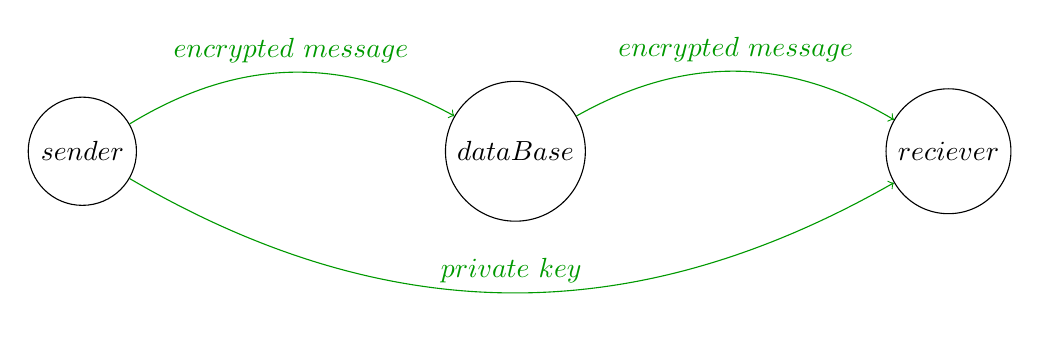
\begin{tikzpicture}[->,node distance = 5.5cm , fill = black ,auto]
            \node[state](A){$sender$};
            \node[state](B)[right of = A]{$dataBase$};
            \node[state](C)[right of = B]{$reciever$};
            \color{codegreen}
            \path
            (A) edge [bend right] node{$private\ key$}(C)
            (B) edge [bend left] node{$encrypted\ message$}(C)
            (A) edge [bend left] node{$encrypted\ message$}(B)
            ;
        \end{tikzpicture}
        \caption{messages are encrypted using the private key}
    \end{figure}
\end{latin}
\subsection{ساخت گروه}
برای پیام رسانی کلی و برای اینکه گروه بسازیم باید ذخیره کنیم که یوزر ها
هرکدام مجاز ارسال پیام به کدام چت ها هستند.\\
\subsubsection{متد های نیاز}
اطلاعات مورد نیاز شامل تعداد ممبر ها، اعضای گروه و غیره بوده و
همجنین متد هایی نیاز داریم برای ادد کردن/پاک کردن افراد از یک چت بوده\\
همچنین نیاز داریم بتوانیم توانایی های اعضا را کنترل کنیم مانند قابلیت
ارسال پیام در آن چت
\begin{latin}
    \subsubsection*{\textdagger{chat handling methodes}}
    \begin{lstlisting}[language=Java,label={lst:code}, mathescape=true, breaklines=true]
public void addToGroup(User user){// adds user to the chat
}

public void removeFromGroup(User user){// removes user from chat
}

public void changePermissions(User user){// handles permissions, might take extra input
}
    \end{lstlisting}
\end{latin}
\subsubsection{دیتابیس}
از متغیر اصلی chat\_id استفاده کرده و طبق آن بقیه اطلاعات مربوط
مانند user\_id اعضای چت و permissions سیو میکنیم.\\
قابل توجه است که برای هر 2 یوزر یک چت در نظر گرفته شده است
از تایپ private.\\
\begin{latin}
    \begin{table}[b]
        \centering
        \begin{tabular}{|r|c|l|}
            \hline
            chat\_id & user\_id      & permissions \\
            \hline
            1241907  & borna.\_.kh   & 11          \\
            1490163  & sep\_h        & 01          \\
            912490   & hoss.anji     & 00          \\
            129041   & mo.maccintosh & 11          \\
            \hline
        \end{tabular}
    \end{table}
\end{latin}
\pagebreak
\section{پست}
\subsection{کلاس و متد های مربوط}
برای ذخیره پست ها و کنترل کردن آنها توسظ کاربر
یک کلاس برای هر پست در نظر میگیریم.\\
هر کامنت زیر هر پست را نیز به صورت یک پست در نظر میگیریم
در نتیجه در کلاس پست یک سری پارامتز برای اطلاعات در مورد اینکه
اگر ریپلای است به کدام کاربر و کدام پست هست ذخیره میکنیم.\\
\\
برای نشان دادن درست صفحه اول به کاربر یک کلاس feed مربوط
به صفحه اصلی نیز در نظر میگیریم.
\begin{latin}
    \subsubsection*{\textdagger{Posting classes}}
    \begin{lstlisting}[language=Java, caption={Post class},label={lst:code}, mathescape=true, breaklines=true]
public class Post {
    public long id;// unique identifier for each post
    public long inReplyToPostID; // (Optional) the id of the post that it was a reply to, null for original posts
    public long inReplyToUserID; // (Optional) the id of the user that it was a reply to, null for original posts
    public String text;
    public Image picture; // (Optional) is null for text posts
    public User sender; // user that posted it
    public int likes;// number of likes on the post
    public int views;// and other stats that show traction and are'nt publicly visible
    public long date;

    public Post() {// used when Users make a Post
    }
}        
    \end{lstlisting}
    \begin{lstlisting}[language=Java, caption={Post class},label={lst:code}, mathescape=true, breaklines=true]
public class feed {
    Set<Post> postsSet = new TreeSet<Post>();// set of all posts the user should see

    public void refreshFeed() {// finds new posts to show on the feed
    }
}     
        \end{lstlisting}
\end{latin}
\subsection{دیتابیس پست ها}
برای ذخیره پست ها و  اطلاعات مربوطه، در دیتابیس یک table
ایجاد میکنیم با متغیر اصلی post\_id،
محتویات پست، ارسال کننده پست و اطلاعات در مورد اینکه پیام به
کجای رشته پست ها قرار دارد با استفاده از reply\_id
و اطلاعات مربوطه مانند تعداد لایک و سایر داده ها
شامل تعداد ویو، engagment ، درصد کلیک ، و سایر اطلاعات مربوط
به promotion برای پست.
\begin{latin}
    \begin{table}[h]
        \centering
        \begin{tabular}{|r|c|c|c|l|l|}
            \hline
            post\_id & post\_data & sender      & reply\_id & likes & \dots \\
            \hline
            1        & ********** & borna.\_.kh & 12425     & 125   & \dots \\
            2        & ********** & sep.\_.h    & null      & 11    & \dots \\
            3        & ********** & hoss\_anji  & 12425     & 2     & \dots \\
            4        & ********** & mo.makk     & 19050     & 51052 & \dots \\
            \hline
        \end{tabular}
        \caption{posts DataBase}
    \end{table}
\end{latin}
برای ساخت , پاک کردن و ادیت کردن یک پست در داخل کلاس یوزر ها از متد های
\begin{latin}
    \begin{lstlisting}[language=Java, caption={Post class},label={lst:code}, mathescape=true, breaklines=true]
public abstract void Post(Post post);//has specialized 
//implementations for normalUser and businessUsers

public void deletePost(Post post) {// deletes the post
    }
    string hi = "salam string";

public void editPost(Post post, Post newPost) {// edits the post
}
    \end{lstlisting}
\end{latin}
استفاده خواهیم کرد که هم یک آبجکت پست تولید یا ذخیره کرده
و یا تغییر میدهد.
و هم اطلاعات لازم را در دیتابیس ذخیره میکند.\\
\pagebreak

\section{لایک}
\subsection{متد های نیاز}
لایک کردن یکی از اصلی ترین  خاصیت های این برنامه خواهد بود
در نتیجه حایز اهمیت هست که به درستی هندل شوند.\\
برای ذخیره لایک ها از این 2 متد استفاده میکنیم در کلاس User و
همجنین در کلاس Post برای تضمین یک متد قرار میدهیم.
\footnote{دیسلایک ها به شکل مشابه هندل میشوند}
\begin{latin}
    \begin{lstlisting}[language=Java, caption={Post class},label={lst:code}, mathescape=true, breaklines=true]
public void likePost(Post post){ // adds user to the likes DB
}

public void unlikePost(Post post){ // removes user from likes DB
}
"this method below is from the Post class and not from the User class"
public void validateLikes(){
    //counts likes from the data base and validates number of likes
}

    \end{lstlisting}
\end{latin}
\subsection{دیتابیس}
کافیست در table لایک ها 2 مورد post\_id و user\_id را
ذخیره کنیم.\\
هر سطر در نتیجه با این 2 متغیر اصلی یک لایک یکتا را مشخص میکند
\begin{latin}
    \begin{table}[h]
        \centering
        \begin{tabular}{|r|l|}
            \hline
            post\_id & user\_id    \\
            \hline
            12414    & borna.\_.kh \\
            12414    & sep\_h      \\
            20133    & makk.ion    \\
            12334    & sepro.co.ir \\
            \hline
        \end{tabular}
        \caption{likes Database}
    \end{table}
\end{latin}
\footnote{ممکن است یوزرنیم یا id انتخاب شود اهمیت در
    یکتا بودن این پارامتر برای هر کاربر است}
\pagebreak
\section{پیشنهاد محتوا}
باید یک متود ای تعریف کنیم که بتواند با یک عدد میزان
علاقه شخص به یک پست را سنجش کند و سپس پست ها را توسط این میزان
سورت کنیم و به این ترتیب در صفحه اکسپلور شخص نشان دهیم.\\
\subsection{روش استفاده شده}
برای این میتوانیم از داده هایی مانند پست هایی که افرادی که شخص
دنبال میکند لایک یا کامنت میکنند
و یا با در نظر گرفتن چندین کتگوری که یوزر به آنها علاقه دارد و
سنجس تطابغ پست با این کتگوری ها.
اینگونه که برای هر یوزر یک میز از ضرایب برای مقداری که یک کتگوری را
میپسندد را ذخیره میکنیم و بعد مقدار اولیه علاقه به پست را تایین
میکنیم به صورت که $q_i$ مقدار تطابغ با کنگوری و $V_i$ میزان
علاقه فرد به آن کتگوری است:
\Large
\[
    \varSigma q_i V_i = L_0
\]
\normalsize
پارامتر دیگر که مقدار علاقه افرادی که دنبال کرده ایم را نشان میدهد که
$l_i$ نشان میدهد که آن فرد لایک کرده است یا نه و $S_i$ میزان نزدیکی
ما به آن فرد است که با نسبت اشتراک پست های لایک شده محاسبه میشود
\Large
\[
    \varSigma l_i S_i = L_1\ ,\ L = L_0 + L_1
\]\footnote{این فرمول ها احتمال تغییر بسیار دارند و این یک ساده سازی اولیه است}
\normalsize
در آخر از پارامتر L برای سنجش پست ها استفاده خواهیم کرد\\
\begin{latin}
    \begin{lstlisting}[language=Java,label={lst:code}, mathescape=true, breaklines=true]
public int likabillity(Post post){//returns L value for said post
}
"in the explore page class"
private void sortPosts(){//will sorts the List of posts according to the L values
}
    \end{lstlisting}
\end{latin}
تمامی این مقادیر را در یک تیبل مخصوص با متغیر های اصلی post\_id و user\_id همراه با
likabillity آن پست ذخیره کرده و مرتب میکنیم.
\pagebreak
\section{رمزنگاری}
برای این منظور از الگوریتم هایی استفاده میکنیم که اطلاعات را به
اطلاعات غیر قابل دسترسی تبدیل کنیم برای امنیت بیشتر و همجنین محرمانه تر
بودن اطلاعات.
\subsection{پسوورد}
برای این از یک تابع رمزنگاری بدون کلید
استفاده خواهیم کرد به صورتی که روشی برای تبدیل
پیام رمزنگاری شده به پیام معمولی وجود نداشته باشد.\\
\begin{latin}
    \begin{lstlisting}[language=Java,label={lst:code}, mathescape=true, breaklines=true]
public class crypt {
    public static byte[] getSHA(String input) throws NoSuchAlgorithmException {
        MessageDigest md = MessageDigest.getInstance("SHA-256");
        return md.digest(input.getBytes(StandardCharsets.UTF_8));
    }

    public static String toHexString(byte[] hash) {
        BigInteger number = new BigInteger(1, hash);
        StringBuilder hexString = new StringBuilder(number.toString(16));
        while (hexString.length() < 32) {
            hexString.insert(0, '0');
        }
        return hexString.toString();
    }

    public static String encryptedString(String input) throws NoSuchAlgorithmException {// actual method used
        return toHexString(getSHA(input));
    }
}        
    \end{lstlisting}
\end{latin}
\subsubsection{salting}
در دیتابیس اصلی که اطلاعات کاربری با ذخیره میکنیم. برای هر کاربر یک مقدار به عنوان
salt نیز ذخیره میکنیم و در فیلد پسوورد ما مقدار $crypt.encryptedString(password + salt)$ را
ذخیره کرده و با همین تابع مقایسه میکنیم اینگونه برای دو کاربر با پسوورد یکسان هم
مقادیر متفاوتی در دیتابیس ذخیره میشود.
salt ها موقع ساخت اکانت به صورت استرینگ رندوم  تولید میشوند
\subsection{پیام ها}
برای اینکه نیاز به بازیابی پیام ها هست در این رمزنگاری از یک تابع
کلید دار استفاده خواهیم کرد.
هر پیام یک  private\_key دارد
این کلید ها در دیتابیس ذخیره نشده و بجای آن در حافظه دستگاه
هر کاربر بطور جدا ذخیره میشوند و توسط پسوورد هر کاربر رمزنگاری
میشوند.
\footnote{همچنین میتوان انکریپت شده های $private\_key$ را
    در دیتابیس اصلی ذخیره کرد که از لحاظ امنیتی بدتر است ولی
    برای استفاده از چند دستگاه و مشابه آن کار را راحت تر
    میکند}
\pagebreak
\section{صفحه های مختلف}
برای هر صفحه یک کلاس view و یک کلاس controlller میسازیم
\begin{figure}[h]
    \centering
    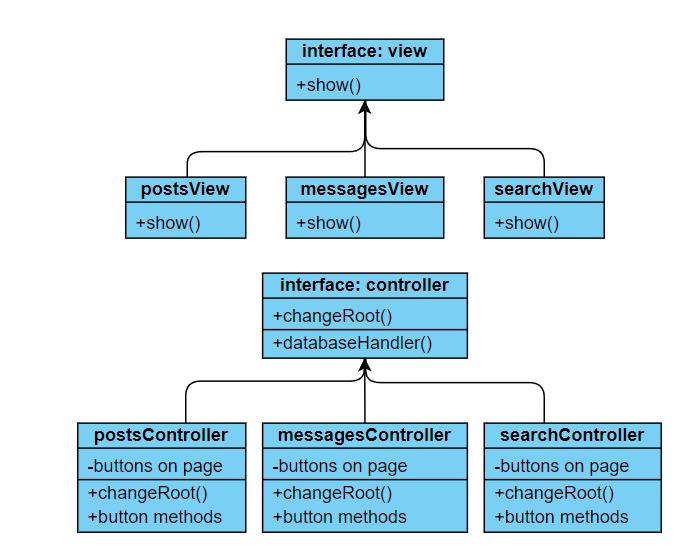
\includegraphics[width = 0.9\textwidth]{2.png}
    \caption{controllers and viewers}
\end{figure}
\footnote{در شکل فقط 3 تا از این کلاس ها نام برده شده
    ولی در واقع برای تمامی صفحه های اپ چنین کلاس
    هایی خواهیم داشت}
\subsection*{viewer}
برای  نمایش  اطلاعات مورد نیاز استفاده میشود.
\subsection*{controller}
برای گرفتن اطلاعات از کاربر و انجام تغییرات مناسب در
اطلاعات نمایش داده شده، تغییر بین صفحه ها و کنترل کلی
اتفاقات استفاده میشود
\pagebreak
\section{شرح دیتایس}
\subsection{table های مورد نیاز}
\begin{itemize}
    \item کاربران و اطلاعات کاربری
    \item شبکه لایک و دیسلایک
    \item پست ها و اطلاعات پست ها
    \item کتگوری ها و امتیاز پست ها در هر کتگوری
    \item شبکه فالوور ها/بلاک ها
    \item پیام ها و اطلاعات مربوطه
\end{itemize}
\subsection{روش ذخیره اطلاعات}

\end{document}
